\setAuthor{Tundmatu autor}
\setRound{lahtine}
\setYear{2004}
\setNumber{G 6}
\setDifficulty{5}
\setTopic{Termodünaamika}

\prob{Aurusaun}
Soojuslikult isoleeritud aurusaun ruumalaga $V = \SI{10}{m^3}$ on temperatuuril $t = \SI{50}{\degreeCelsius}$ ning suhtelise õhuniiskusega (veeauru tiheduse ning küllastunud veeauru tiheduste suhe) $r = \SI{80}{\%}$. Saunas lülitatakse sisse keeva veega töötav küttekeha. $\tau = \SI{20}{min}$ möödudes hakkab saunas kondenseeruma vesi, kusjuures selleks ajaks on küttekehas aurustunud $m = \SI{620}{g}$ vett. Vee keemissoojus on $L = \SI{2.3e6}{J/kg}$, õhu keskmine erisoojus $c=\SI{1000}{J.kg^{-1}.\degreeCelsius^{-1}}$, tihedus $\rho = \SI{1.3}{kg/m^3}$. Küllastunud veeauru tiheduse sõltuvus temperatuurist on toodud graafikul. Võite ignoreerida aurusauna õhuvahetuse mõju õhuniiskusele.\\
\osa Mis oli sauna temperatuur hetkel, mil vesi kondenseeruma hakkas?\\
\osa Missuguse kasuteguriga küttekeha vett aurustas?\\
\osa Mis on küttekeha võimsus?
\begin{center}
	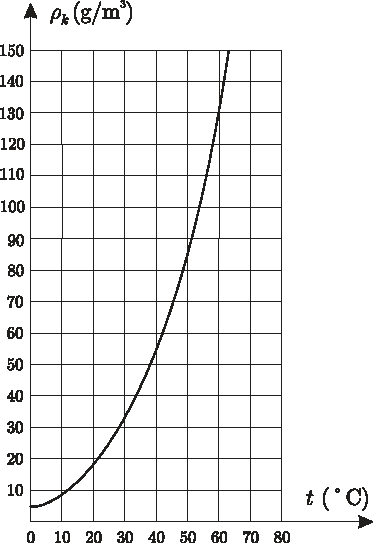
\includegraphics[width=0.5\linewidth]{2004-lahg-06-yl.pdf}
\end{center}

\hint
\osa Kuna ülesandes eeldatakse, et aurusauna õhuvahetus ei mõjuta õhus olevat niiskust, kehtib vee massi jäävus. Esialgne absoluutne vee tihedus saunas on leitav algandmetest (ja graafikult lugedes) ning vee tiheduse muut on antud aurustuva vee massi kaudu.

\osa\osa Kehtib energia jäävuse seadus. Küttekeha soojus läheb nii eksisteeriva õhu soojenemisesse kui ka vee keetmisesse.

\solu
Graafikult loeme, et $t=\SI{50}{\degreeCelsius}$ juures on küllastatud auru tihedus $\rho_{k}=\SI{85}{g/m^3}$. Seega on absoluutne õhuniiskus saunas
$$
f=r \rho_{k}=\SI{68}{g/m^3}.
$$
Kui ruumis ruumalaga $V$ aurustub vesi massiga $m$, siis tõuseb absoluutne niiskus
$$
\Delta f=\frac{m}{V}=\frac{620}{10}=\SI{62}{g/m^3}
$$
võrra ja on kokku
$$
f^{\prime}=f+\Delta f=\SI{130}{g/m^3}.
$$
Kuna ruumis hakkab kondenseeruma vesi, siis järelikult on aur ruumis küllastunud, seega absoluutne niiskus $f^{\prime}$ on ühtlasi ka küllastunud auru tihedus sellel temperatuuril:
$f^{\prime}=\rho_{k}^{\prime} .$ Kuna igale temperatuurile vastab ainult üks kindel küllastunud auru tiheduse väärtus (mida kõrgem on temperatuur, seda tihedam on küllastunud auru tihedus), siis tihedam küllastunud aur tähendab ühtlasi ka kõrgemat temperatuuri ruumis. Graafikult leiame, et sellise küllastunud auru tihedusele vastab temperatuur $t^{\prime}=60^{\circ} \mathrm{C}$. Temperatuuri muut on $\Delta t=\SI{10}{\degreeCelsius}$. Kokku kulub sooja $M c \Delta t+m L$, millest aurustumiseks kulub $m L$. Siin $M$ on õhu mass, mille me leiame valemist $M=\rho V$, kus $V$ on sauna ruumala. Seega on küttekeha kasutegur aurustumise suhtes
$$
\eta=\frac{m L}{m L+\rho V c \Delta t} \approx \SI{91,6}{\%}
$$
ning küttekeha võimsus on
$$
P=\frac{m L+\rho V c \Delta t}{\tau} \approx \SI{1300}{W}.
$$

\probend